\documentclass[a4paper,12pt]{amsart}

\usetheme[progressbar=frametitle]{metropolis}
\metroset{block=fill}

\subtitle{NTIN071 Automata and Grammars}
\author{Jakub Bulín (KTIML MFF UK)}

\date{Spring 2025\\ 
    \vspace{1in} 
    \begin{flushleft}
        \it \footnotesize * Adapted from the Czech-lecture slides by Marta Vomlelová with gratitude. The translation, some modifications, and all errors are mine.
    \end{flushleft}
}

%% packages

\usepackage{amsmath}
\usepackage{amssymb}
\usepackage{amsthm}
\usepackage{cancel}
\usepackage{color}
\usepackage{colortbl}
\usepackage{forest}
\usepackage[utf8x]{inputenc}
\usepackage{multicol}
\usepackage{multirow}

%% colors
\definecolor{Gray}{gray}{0.9}

%% TikZ
\usepackage{tikz}
    \usetikzlibrary{
        automata,
        arrows,
        backgrounds,
        decorations.pathmorphing,
        fit,
        positioning,
        shapes,
        shapes.geometric,
        tikzmark
    } 
    \tikzset{>=stealth',shorten >=1pt,auto,node distance=2cm}
    \tikzset{initial text={}}
    \tikzset{elliptic state/.style={draw,ellipse}}

%% amsthm
\theoremstyle{plain}
    \newtheorem*{algorithm}{Algorithm}    
    \newtheorem*{observation}{Observation}
    \newtheorem*{proposition}{Proposition}

\theoremstyle{remark}
    \newtheorem*{exercise}{Exercise}
    \newtheorem*{remark}{Remark}

%% macros
\DeclareMathOperator{\RegE}{RegE}
\DeclareMathOperator{\RL}{RL}

% Just for Lecture 2
\newcommand{\x}{$\times$}
\newcommand{\nx}{\ }


\begin{document}

\thispagestyle{empty}

\section*{NTIN071 A\&G: Cvičení 7 -- Formální gramatiky, regulární a bezkontextové gramatiky, bonus: dvousměrné automaty}

% po 6. a 7. přednášce
% jaro 2024

\medskip

\noindent\emph{Vyřešte nejprve 1a-d, 2, 3, 4ab (zbytek je na procvičení, bonusová sekce o dvousměrných automatech v testu nebude).}

\medskip


\medskip\begin{problem}[Konstrukce gramatik]

    Navrhněte gramatiky (co nejvyššího typu), které generují následující jazyky (nad abecedou $\Sigma=\{a,b\}$, není-li řečeno jinak).

    \begin{multicols}{2}
    \begin{enumerate}[(a)]    
        \item $L=\Sigma^*$
        \item $L=\{w\mid |w|_b\text{ je sudý}\} $
        \item $L=\{ww^R\mid w\in \Sigma^*\} $
        \item $L=\{a^{2i}b^j\mid i\leq j\}$
        \item $L=\{w\mid |w|_a = 2|w|_b\}$
        \item $L = \{a^ib^jc^k\mid i = j\text{ nebo }j = k\}$
    
    \end{enumerate}
    \end{multicols}

\end{problem}


\begin{problem}[Z konečného automatu na gramatiku]
 
    Pro následující konečný automat nalezněte ekvivalentní gramatiku. V jaké třídě Chomského hierarchie se budete pohybovat?

	\begin{center}
        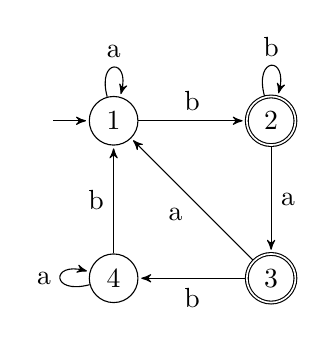
\begin{tikzpicture}[>=stealth',shorten >=1pt,auto,node distance=2cm]
        		\tikzset{every state/.style={minimum size=0.2cm}}
        			
        			\node[initial,state]  (a1)      {1};
        			\node[state,accepting] (b1)  [right of=a1]    {2};
        				\node[state,accepting] [below of=b1](c1)      {3};
        				\node[state] [below of=a1](d1)      {4};
        		\path[->]
        				(a1)  edge  node {b} (b1)
        				(a1)  edge[loop above]  node {a} (a1)
        				(b1)  edge[loop above]  node {b} (b1)
        				(d1)  edge[loop left]  node {a} (d1)
        				(b1)  edge  node {a} (c1)
        				(c1)  edge  node {a} (a1)
        				(c1)  edge  node {b} (d1)
        				(d1)  edge  node {b} (a1)
        				;
        	\end{tikzpicture}
    \end{center}

\end{problem}


\medskip\begin{problem}[Z regulární gramatiky na konečný automat] 
    
    Pro následující pravou lineární gramatiku sestrojte ekvivalentní konečný automat: $G=(\{S,A,B,C\},\{a,b\},\mathcal P,S)$, kde $\mathcal P$ sestává z následujících pravidel: 

    \medskip

    \begin{center}
        \begin{tabular}{l}
        $S\rightarrow abS\mid babA\mid \lambda $\\
        $A\rightarrow abA\mid aB \mid  bC$\\
        $B\rightarrow abS\mid B\mid bC\mid \lambda $\\
        $C\rightarrow aab\mid A\mid aA\mid \lambda $
        \end{tabular}
    \end{center}

\end{problem}


\medskip\begin{problem}[Testování vlastností bezkontextových jazyků]
    Vymyslete (co nejefektivnější) algoritmus, který rozhodne, zda daná bezkontextová gramatika splňuje danou vlastnost:

    \medskip
    
    \begin{enumerate}[(a)]
        \item $L(G)\neq\emptyset$
        \item $\lambda\in L(G)$
        \item $L(G)$ je konečný jazyk
    \end{enumerate}

\end{problem}


\medskip\begin{problem}[Malé gramatiky generující velké (konečné) jazyky]
    
    Najděte posloupnost bezkontextových gramatik $G_1,G_2,G_3,\dots$ (nad danou abecedou $\Sigma$) takových, že $G_n$ generuje právě všechna slova délky $\leq 2^n$ (a žádná jiná), a přitom velikost $G_n$ (pro jednoduchost počet symbolů v tělech produkčních pravidel) je v $O(n)$.
    
    %X_1 \to X_2_X2, X_2 \to X_3X_3,\dots, X_{n−1}\to X_nX_n, X_n\to aa|a|\lambda

\end{problem}


\bigskip


\section*{Bonus: Dvousměrné automaty}


\medskip\begin{problem}[Dvousměrný automat, převod na jednosměrný]

    Mějme následující dvousměrný automat.

    \begin{multicols}{2}

    \begin{center}
        \begin{tabular}{ r | c c }
        & a & b \\
        \hline
        $\to\ast p$ & $p,1$ & $q,-1$ \\
        $q$ & $r,1$ & \\
        $r$ & & $p,1$
        \end{tabular}
    \end{center}

    \begin{center}
        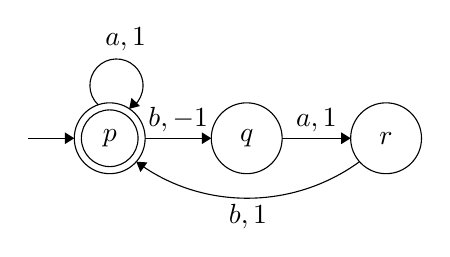
\begin{tikzpicture}[scale=0.15]
            \tikzstyle{every node}+=[inner sep=0pt]
            \draw [black] (10.1,-9.7) circle (3);
            \draw (10.1,-9.7) node {$p$};
            \draw [black] (10.1,-9.7) circle (2.4);
            \draw [black] (21.7,-9.7) circle (3);
            \draw (21.7,-9.7) node {$q$};
            \draw [black] (33.5,-9.7) circle (3);
            \draw (33.5,-9.7) node {$r$};
            \draw [black] (3.2,-9.7) -- (7.1,-9.7);
            \fill [black] (7.1,-9.7) -- (6.3,-9.2) -- (6.3,-10.2);
            \draw [black] (9.129,-6.874) arc (226.70189:-61.29811:2.25);
            \draw (11.45,-2.35) node [above] {$a,1$};
            \fill [black] (11.75,-7.21) -- (12.66,-6.97) -- (11.94,-6.28);
            \draw [black] (13.1,-9.7) -- (18.7,-9.7);
            \fill [black] (18.7,-9.7) -- (17.9,-9.2) -- (17.9,-10.2);
            \draw (15.9,-9.2) node [above] {$b,-1$};
            \draw [black] (24.7,-9.7) -- (30.5,-9.7);
            \fill [black] (30.5,-9.7) -- (29.7,-9.2) -- (29.7,-10.2);
            \draw (27.6,-9.2) node [above] {$a,1$};
            \draw [black] (31.254,-11.682) arc (-53.92224:-126.07776:16.054);
            \fill [black] (12.35,-11.68) -- (12.7,-12.56) -- (13.29,-11.75);
            \draw (21.8,-15.26) node [below] {$b,1$};
        \end{tikzpicture}
    \end{center}

    \end{multicols}

    \begin{enumerate}[(a)]
        \item Určete jakyk přijímaný tímto automatem.
        \item Určete funkce $f_u$ a kongruenci $\sim$ pro všechna slova délky nejvýše $4$.
        \item Převeďte ho na ekvivalentní jednosměrný konečný automat.
    \end{enumerate}

\end{problem}


\medskip\begin{problem}[Bez dvousměrných automatů to jde těžko]
    
    Pro daný DFA $A$ navrhněte nedeterministický konečný automat přijímající jazyk $L'=\{\#w\#\ |\ ww^R\in L(A)\}$. Přitom nevyužívejte znalosti dvousměrných automatů.

\end{problem}


\medskip\begin{problem}[Konstrukce dvousměrného automatu]
    
    Nechť $L$ je regulární jazyk nad abecedou $\Sigma$ rozpoznávaný konečným automatem $A$ a $\#\notin\Sigma$. Sestrojte dvousměrný konečný automat rozpoznávající daný jazyk: 
    
    \begin{enumerate}[(a)]
        \item $L' = \{\#w\#\mid ww^R \in L\}$
        \item $L' = \{\#w\#\mid (\exists u \in\Sigma^*)\, wu \in L\ \& \ |w|=|u|\}$
    \end{enumerate}

\end{problem}


\end{document}
